% !TEX root = thesis.tex

%% \usepackage{cmbright}                          % serifenlose computer modern fonts

\usepackage[quiet]{fontspec}
\setmonofont[Contextuals={Alternate}]{Fira Code}
\usepackage[T1]{fontenc}                       % T1 fonts für gute pdf-Ausgabe
% \usepackage[utf8]{inputenc}                    % wegen deutschen Umlauten
\usepackage[automark]{scrpage2}                % Koma Headers

% \usepackage[english]{babel}

\usepackage{nag}                               % warn user on outdated packages
\usepackage[linktocpage, hidelinks]{hyperref}  % links in pdf, thumbnails
\usepackage{soul}                              % emphasizing text, underlining
\usepackage[onehalfspacing]{setspace}          % 1.5, change line spaces by \singlespacing \doublespacing

%% tables
\usepackage{multicol}                          % multiple columns in tables
\usepackage{multirow}                          % multiple rows in tables
\usepackage[margin=10pt,labelfont=bf]{caption} % table headers
\usepackage{hhline}                            % horizontal lines
\usepackage{longtable}                         % pagebreak tables
\usepackage{booktabs}                          % bold table lines, e.g. \toprule
\usepackage{tabularx}                          % neue Tabular-Umgebung

%% math, symbols
\usepackage{amsmath}                           % AMS Math like brackets, integrals...
\usepackage{amssymb}                           % AMS-Symbols v2.0
\usepackage{fixmath}                           % big greek letters italic in math mode
\usepackage{array}                             % matrices
\usepackage[per-mode=symbol]{siunitx}                           % includes nicefrac, nicer fracs for one line, SI-Units
\DeclareSIUnit{\bits}{bits}
\usepackage[integrals]{wasysym}                % for integrals like \oiint


\usepackage{microtype}                         % character protruding, font expansion - instead of pdfcprot
\usepackage{graphicx}                          % include graphics
\usepackage{wrapfig}                           % graphics in text
\usepackage{floatflt}                          % graphics/tables in text
\usepackage{rotating}                          % rotating elements

\usepackage[svgnames]{xcolor}                  % colors for listings
\usepackage{psfrag}                            % Text in .eps Grafiken ersetzen
\usepackage{float}
\usepackage[european]{circuitikz}
\usepackage{pgfplots}
 \pgfplotsset{compat=1.5}
\renewcommand{\rmdefault}{pplx}
\usepackage{eulervm}                           % math font


\usepackage{subcaption}  % subcaptions

\usepackage{lipsum} % blind text
\usepackage[noabbrev]{cleveref} % references

\usepackage[
    acronym,
    % counter=section,
    style=longheader,
    indexonlyfirst,
    nopostdot]{glossaries-extra}
\setabbreviationstyle[acronym]{long-short} % first occurence long, rest short
\renewcommand*{\acrshort}[1][]{\glsxtrshort[noindex,#1]} % acrshort -> no index

% code
\usepackage[cachedir=out/_minted-\jobname]{minted}
\usemintedstyle{colorful}

\usepackage{bytefield}

\newcommand{\xor}{\ensuremath \veebar}

\usepackage{nicefrac}
\usepackage{xcolor}

\usetikzlibrary{external}
\tikzexternalize[prefix=tikz_out/]

\makeatletter
\DeclareRobustCommand{\skippedwords}[1][1ex]{%
  \setlength{\units@wide}{\bf@bitwidth * \bits@wide}%
  \setlength{\units@high}{1pt * \ratio{\units@wide}{9.0pt}}%
  \setlength{\units@tall}{#1 + \units@high}%
  \edef\num@wide{\strip@pt\units@wide}%
  \edef\num@tall{\strip@pt\units@tall}%
  \edef\num@high{\strip@pt\units@high}%
  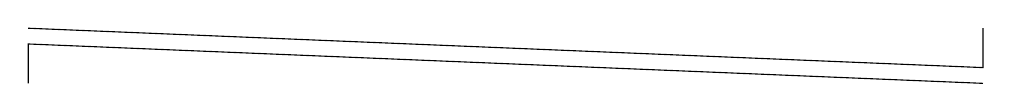
\begin{tikzpicture}
    \draw (\linewidth,0) -- (0,0.5) -- (0,0);
    \draw (0,0.7) -- (\linewidth,0.2) -- (\linewidth,0.7);
  \end{tikzpicture}
  \ifcounting@words
    \inc@bytefield@height{\unitlength * \real{\num@tall}}%
    \global\counting@wordsfalse
  \fi}
  \makeatother

% \usepackage[datesep=., style=ddmmyyyy]{datetime2}
\newcommand{\leadingzero}[1]{\ifnum #1<10 0\the#1\else\the#1\fi}
\renewcommand{\today}{\leadingzero{\day}.\leadingzero{\month}.\the\year}


\usepackage[
    backend=biber,
    style=numeric,
  ]{biblatex}

 \addbibresource{bib.bib}

% \usepackage[all]{nowidow}
\usepackage[bottom]{footmisc}
\usepackage{csquotes}
\usepackage{etoolbox}

\preto\chapter{
  % \glsreset{RDMA}
  % \glsreset{RoCEv2}
  % \glsreset{FPGA}
  % \glsreset{ASIC}
  % \glsreset{UDP}
  % \glsreset{TCP}
  \glsreset{AXI}
  \glsreset{CPU}
  \glsreset{SIFT}
  \glsreset{PCB}
  % \glsreset{DMA}
  % \glsreset{RAM}
  \glsreset{SRAM}
  \glsreset{IB}
  \glsreset{IP}
  \glsreset{DSP}
  \glsreset{BRAM}
  \glsreset{EPROM}
  \glsreset{CLB}
  \glsreset{LUT}
  \glsreset{MUX}
  \glsreset{MTU}
  \glsreset{PSN}
  \glsreset{CM}
  \glsreset{RC}
  \glsreset{UD}
  \glsreset{ICRC}
  \glsreset{CRC}
  \glsreset{IANA}
  \glsreset{TTL}
  \glsreset{QP}
  \glsreset{BTH}
  \glsreset{DETH}
  \glsreset{MAD}
  \glsreset{RNR}
  \glsreset{ARI}
  \glsreset{MSB}
  \glsreset{LSB}
  \glsreset{LRH}
  \glsreset{GRH}
  \glsreset{AETH}
  \glsreset{RETH}
  \glsreset{NAK}
  \glsreset{MAC}
  \glsreset{DDR}
  % \glsreset{FIFO}
  % \glsreset{VHDL}
  % \glsreset{VHSIC}
  \glsreset{LFSR}
  \glsreset{DUT}
  \glsreset{ALM}
  \glsreset{LAB}
  \glsreset{MLAB}
  \glsreset{OS}
}
